\documentclass{beamer}

\usepackage{wrapfig}
\usepackage[linesnumbered,ruled,vlined]{algorithm2e}
\usepackage{tikz}
\usepackage{pgfplots}
\usepackage{graphicx}
\pgfplotsset{compat=1.18}
\usepackage{amsmath}
\usetikzlibrary{intersections, through, calc}

\renewcommand{\algorithmcfname}{Algorithmus}

% Theme and colors
\usetheme{Singapore} % Clean layout
\usecolortheme{default}

% Custom colors
\definecolor{DarkBlue}{RGB}{10, 25, 47} % Dark navy
\definecolor{FrameTextColor}{RGB}{255,255,255}

% Set background canvas color (header/footer)
\setbeamercolor{frametitle}{bg=DarkBlue, fg=FrameTextColor}
\setbeamercolor{title}{bg=DarkBlue, fg=FrameTextColor}
\setbeamercolor{author}{fg=FrameTextColor}
\setbeamercolor{date}{fg=FrameTextColor}
\setbeamercolor{section in head/foot}{bg=DarkBlue, fg=FrameTextColor}
\setbeamercolor{subsection in head/foot}{bg=DarkBlue, fg=FrameTextColor}
\setbeamercolor{footline}{bg=DarkBlue, fg=FrameTextColor}
\setbeamercolor{headline}{bg=DarkBlue, fg=FrameTextColor}

% Remove navigation symbols
\setbeamertemplate{navigation symbols}{}

% Title page setup
\title[Die Geometrische Brownsche Bewegung und Anwendungen]{Die Geometrische Brownsche Bewegung und Anwendungen}
\author{Fabian Schuller}
\date{\today}

% Custom footline (optional)
\setbeamertemplate{footline}{
  \leavevmode%
  \hbox{%
  \begin{beamercolorbox}[wd=0.7\paperwidth,ht=2.5ex,dp=1ex,left]{author in head/foot}%
    \hspace{1em}\insertshortauthor{} - \insertshorttitle{}
  \end{beamercolorbox}%
  \begin{beamercolorbox}[wd=0.3\paperwidth,ht=2.5ex,dp=1ex,right]{date in head/foot}%
    \insertframenumber{} / \inserttotalframenumber\hspace{1em}
  \end{beamercolorbox}}%
  \vskip0pt%
}

% Begin document
\begin{document}

\section{Einleitung}

\begin{frame}
  \titlepage
\end{frame}

\begin{frame}{Inhalt}
  \begin{itemize}
    \item Grundlagen zu Stochastischen Prozessen und der Brownschen Bewegung
    \item Herleitung der geometrischen Brownschen Bewegung aus dem Binomialmodell
    \item Modellierung von Finanzzeitreihen mit der geometrischen Brownschen Bewegung
    \item Bewertung von Aktienoptionen mit Black Scholes
  \end{itemize}
\end{frame}

\section{Die Brownsche Bewegung}

\begin{frame}{Stochastische Prozesse}
    \begin{itemize}
      \item Zeitdiskrete Modelle: Zufallsspaziergang, Binomialmodell
      \item Zeitstetige Grenzprozesse: Brownsche Bewegung als Limit
      \item Filtration, bedingter Erwartungswert, Adaptierung (Information über Zeit)
    \end{itemize}
\end{frame}

\begin{frame}{Die diskrete Brownsche Bewegung}
  \begin{itemize}
    \item Konstruktion durch aufsummierte unabhängige Normalvariablen
    \item Skaliertes Interpolationsverfahren (N-ter Ordnung) ($\rightarrow$ Varianz $\to$ t)
    \item Martingal-Eigenschaft und Varianzwachstum linear in der Zeit
  \end{itemize}
  \begin{figure}
    \centering
  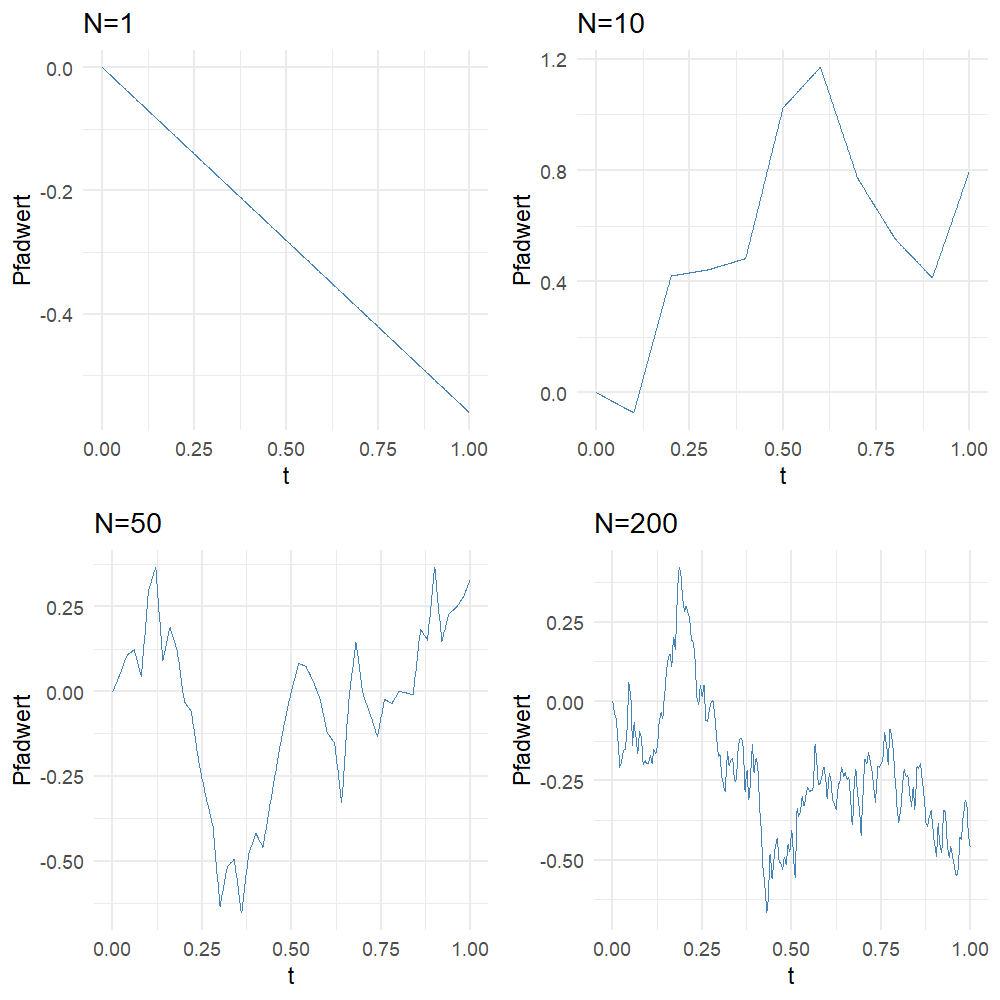
\includegraphics[width=0.4\textwidth]{../thesis/images/disrete_bb.png}
  \end{figure}
\end{frame}

\begin{frame}{Die Brownsche Bewegung}
  \begin{itemize}
  \item Klassische Axiome
    \begin{itemize}
      \item $W_0=0$, Pfade fast-sicher stetig
      \item unabhängige, stationäre Normalinkremente
    \end{itemize}
  \item Brownsche Bewegung als Grenzwert
    \begin{itemize}
      \item Donsker / Zentrale Grenzwertsatz für Prozesse
      \item Existenz der endlich-dimensionalen Verteilungen und Kontinuität
    \end{itemize}
\end{itemize}
\end{frame}

\begin{frame}{Kovarianzstruktur der Brownschen Bewegung}
  \begin{itemize}
    \item Kovarianz: $\mathrm{Cov}(W_s,W_t)=\min(s,t)$
  \item Unabhängigkeit der Inkremente $\Rightarrow$ Varianz wächst linear
    \item Grundlage für Simulation und Modellierung von Zeitreihen
  \end{itemize}
  \begin{figure}
    \centering
  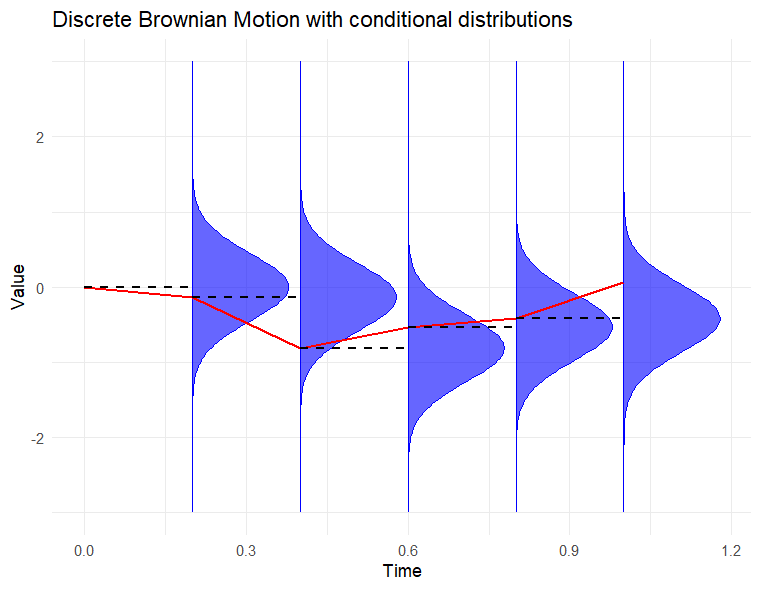
\includegraphics[width=0.48\textwidth]{../thesis/images/bb_with_cov.png}
  \end{figure}
\end{frame}

\begin{frame}{Eigenschaften der Brownschen Bewegung}
  \begin{itemize}
      \item Martingal-Eigenschaft
      \item stationäre, unabhängige Inkremente, Normalverteilung
      \item Pfade zwar nicht differenzierbar, aber stetig
      \item Somit eignet sich die Brownsche Bewegung zur Modellierung von Rauschen
  \end{itemize}
\end{frame}

\section{Die geometrische Brownsche Bewegung}

\begin{frame}{Diskretes Modell}
  \begin{itemize}
      \item Multiplikatives Modell: $S_{k+1}=S_k(1+X_{k+1})$
      \item Annahme: $X_{k+1}=\mu\Delta t+\sigma\sqrt{\Delta t}\,\varepsilon_{k+1}$
      \item Dies kann man als diskrete stochastische Differenzengleichung (SDE) interpretieren.
      \item Genauer: Euler--Maruyama-Approximation der SDE $$dS_t = \mu S_t\,dt + \sigma S_t\,dW_t$$
  \end{itemize}
\end{frame}

\begin{frame}{Geschlossene Formel}
  \begin{itemize}
      \item Geschlossene Lösung der SDE / Grenzwert der diskreten Übergangsvariablen
      \item $S_T = S_0 \exp\big((\mu-\tfrac12\sigma^2)T + \sigma W_T\big)$
      \item $S_T$ ist log-normalverteilt; Erwartungswert und Varianz bekannt
  \end{itemize}
\end{frame}

\begin{frame}{Beweisskizze}
  \begin{itemize}
      \item Logarithmierung: $\log S_n = \log S_0 + \sum \log(1+X_j)$
      \item Taylor-Entwicklung bis 2. Ordnung, Quadratterm liefert $-\tfrac12\sigma^2T$
      \item ZGWS f. Summe der Zufallsvariablen $\Rightarrow \sigma W_T$; GGZ f. Quadratterm
  \end{itemize}
\end{frame}

\begin{frame}{Eigenschaften}
  \begin{itemize}
      \item Positivität: $S_t>0$ fast sicher
      \item Log-Normalverteilung: einfache Momente für Risikoanalyse
      \item Skalierungseigenschaften; analytische Preise für einfache Derivate
  \end{itemize}
\end{frame}

\section{Anwendungen}

\begin{frame}{Kalibrierung}
  \begin{itemize}
      \item Schätzung von $\mu,\sigma$ über Log-Returns
      \item Konfidenzintervalle und Unsicherheitsschätzung (Bootstrap)
  \end{itemize}
\end{frame}

\begin{frame}{Simulation}
  \begin{itemize}
      \item Exakte Pfadsimulation für GBM via geschlossene Formel
      \item Monte-Carlo-Simulation für Optionspreise und Konfidenzbänder
      \item Numerik: Euler--Maruyama für verallgemeinerte Modelle (CEV etc.)
  \end{itemize}
  \begin{figure}
    \centering
  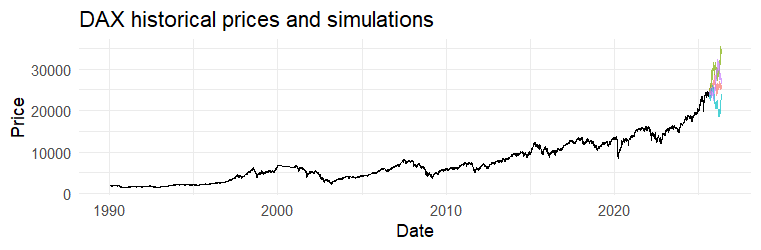
\includegraphics[width=0.48\textwidth]{../thesis/images/dax_monte_carlo.png}
  \end{figure}
\end{frame}

\begin{frame}{Backtests}
  \begin{itemize}
      \item Evaluierung von Handelsstrategien auf historischen Daten (DAX, Lufthansa, ...)
      \item Vergleich von Modellen (GBM vs. CEV) mittels Backtests und Performance-Metriken
      \item Visualisierung der Backtests und Confidence Bands
  \end{itemize}
  \begin{figure}
    \centering
  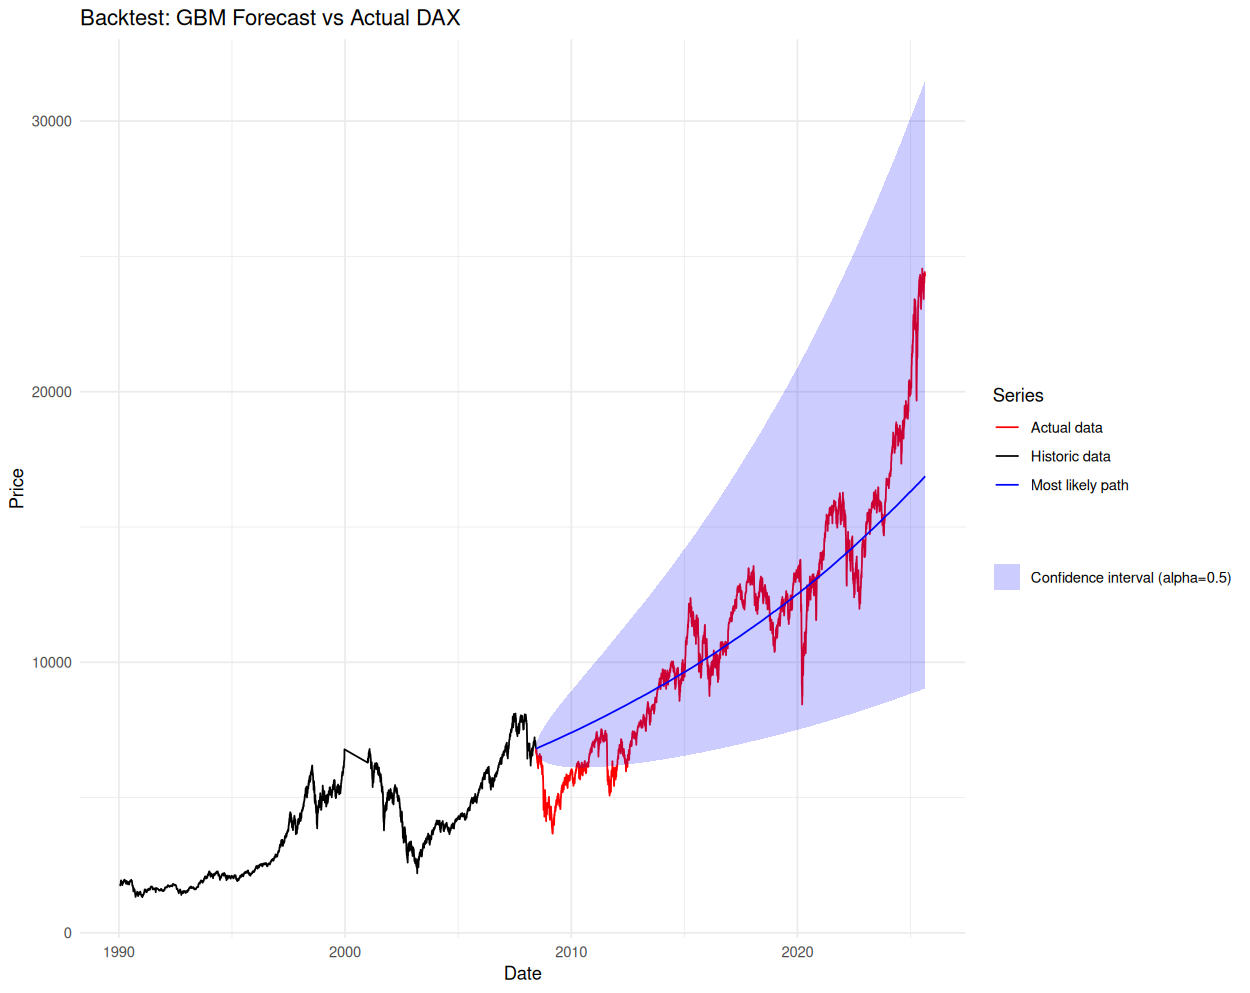
\includegraphics[width=0.48\textwidth]{../thesis/images/dax_backtest.png}
  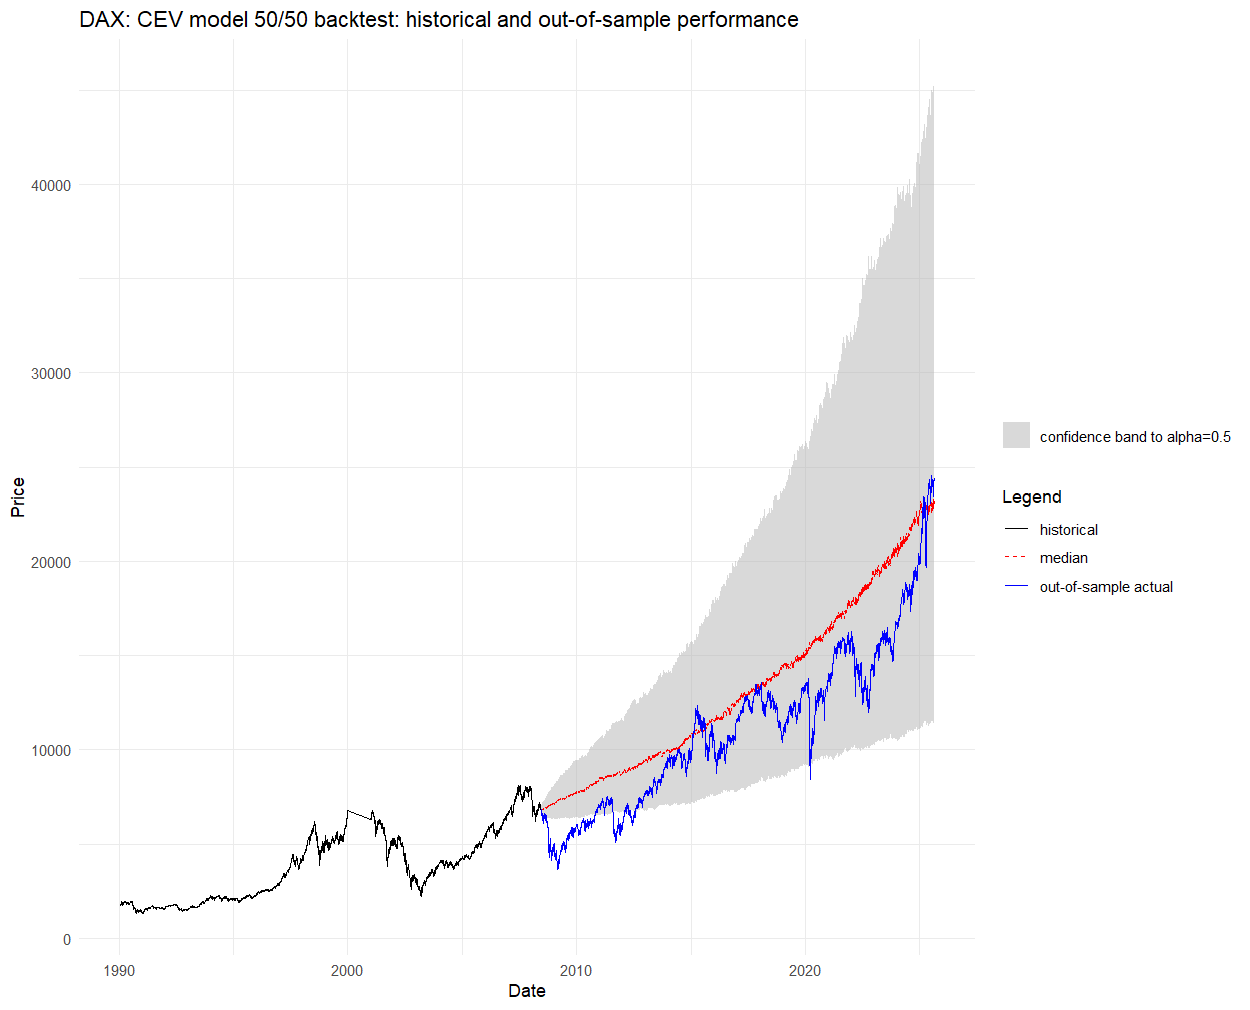
\includegraphics[width=0.48\textwidth]{../thesis/images/cev_dax_backtest.png}
  \end{figure}
\end{frame}

\section{Black-Scholes}

\begin{frame}{Optionen}
  \begin{itemize}
      \item Europäische Call- und Put-Option: Recht, nicht Pflicht
      \item Auszahlung: $\max(S_T-K,0)$ (Call), $(K-S_T)^+$ (Put)
      \item Unterscheidung: europäisch vs. amerikanisch (Ausübungsrechte)
  \end{itemize}
\end{frame}

\begin{frame}{Risikoneutrale Bewertung}
  \begin{itemize}
      \item Diskontierter Aktienkurs ist unter dem risikoneutralen Maß $Q$ ein Martingal
      \item Erwartungswert unter $Q$ des diskontierten Auszahlungsstroms gibt den fairen Preis
      \item Hedging-Interpretation: Replikation via dynamischem Portfolio (Delta-Hedging)
  \end{itemize}
\end{frame}

\begin{frame}{Der faire Preis von Optionen}
  \begin{itemize}
      \item Für europäische Calls: Black-Scholes-Formel
      \item $C = S_0\Phi(d_1) - Ke^{-rT}\Phi(d_2)$ mit $d_{1,2}$ standardmäßig definiert
      \item Keine Arbitrage, perfekte Replikation unter Modellannahmen
  \end{itemize}
\end{frame}

\begin{frame}{Das Black-Scholes Modell}
  \begin{itemize}
      \item Modellannahmen: GBM für Underlier, konstante $r,\sigma$, keine Transaktionskosten
      \item PDE-Herleitung führt zur geschlossenen Preislösung für europäische Optionen
      \item Praktische Limitationen: Volatilitätsstruktur, Marktfriktionen
  \end{itemize}
\end{frame}

\begin{frame}{Beispiele}
  \begin{itemize}
      \item Numerische Bewertung vs. geschlossene Formel: Vergleich für DAX-Calls
      \item Monte-Carlo- vs. Black-Scholes-Ergebnisvergleiche
  \end{itemize}
  \begin{figure}
    \centering
  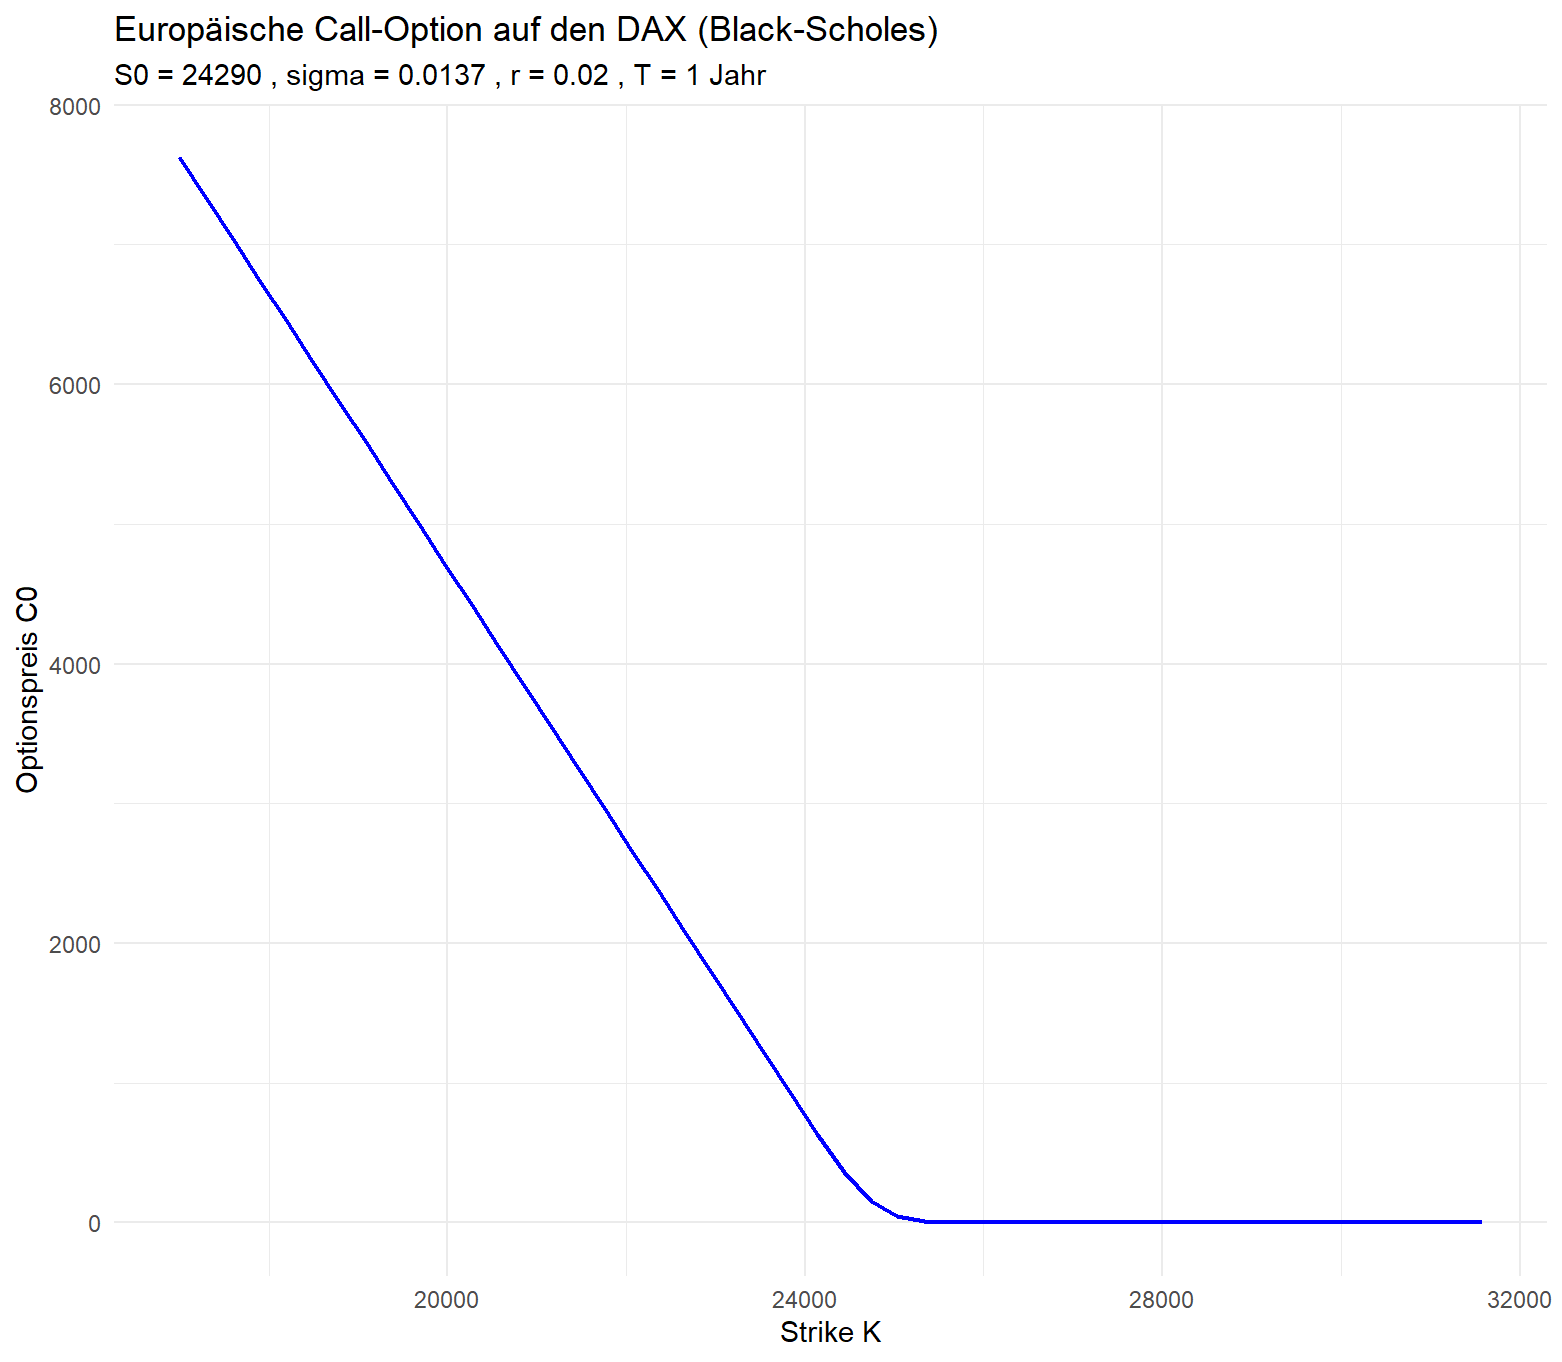
\includegraphics[width=0.48\textwidth]{../thesis/images/call_dax_bs.png}
  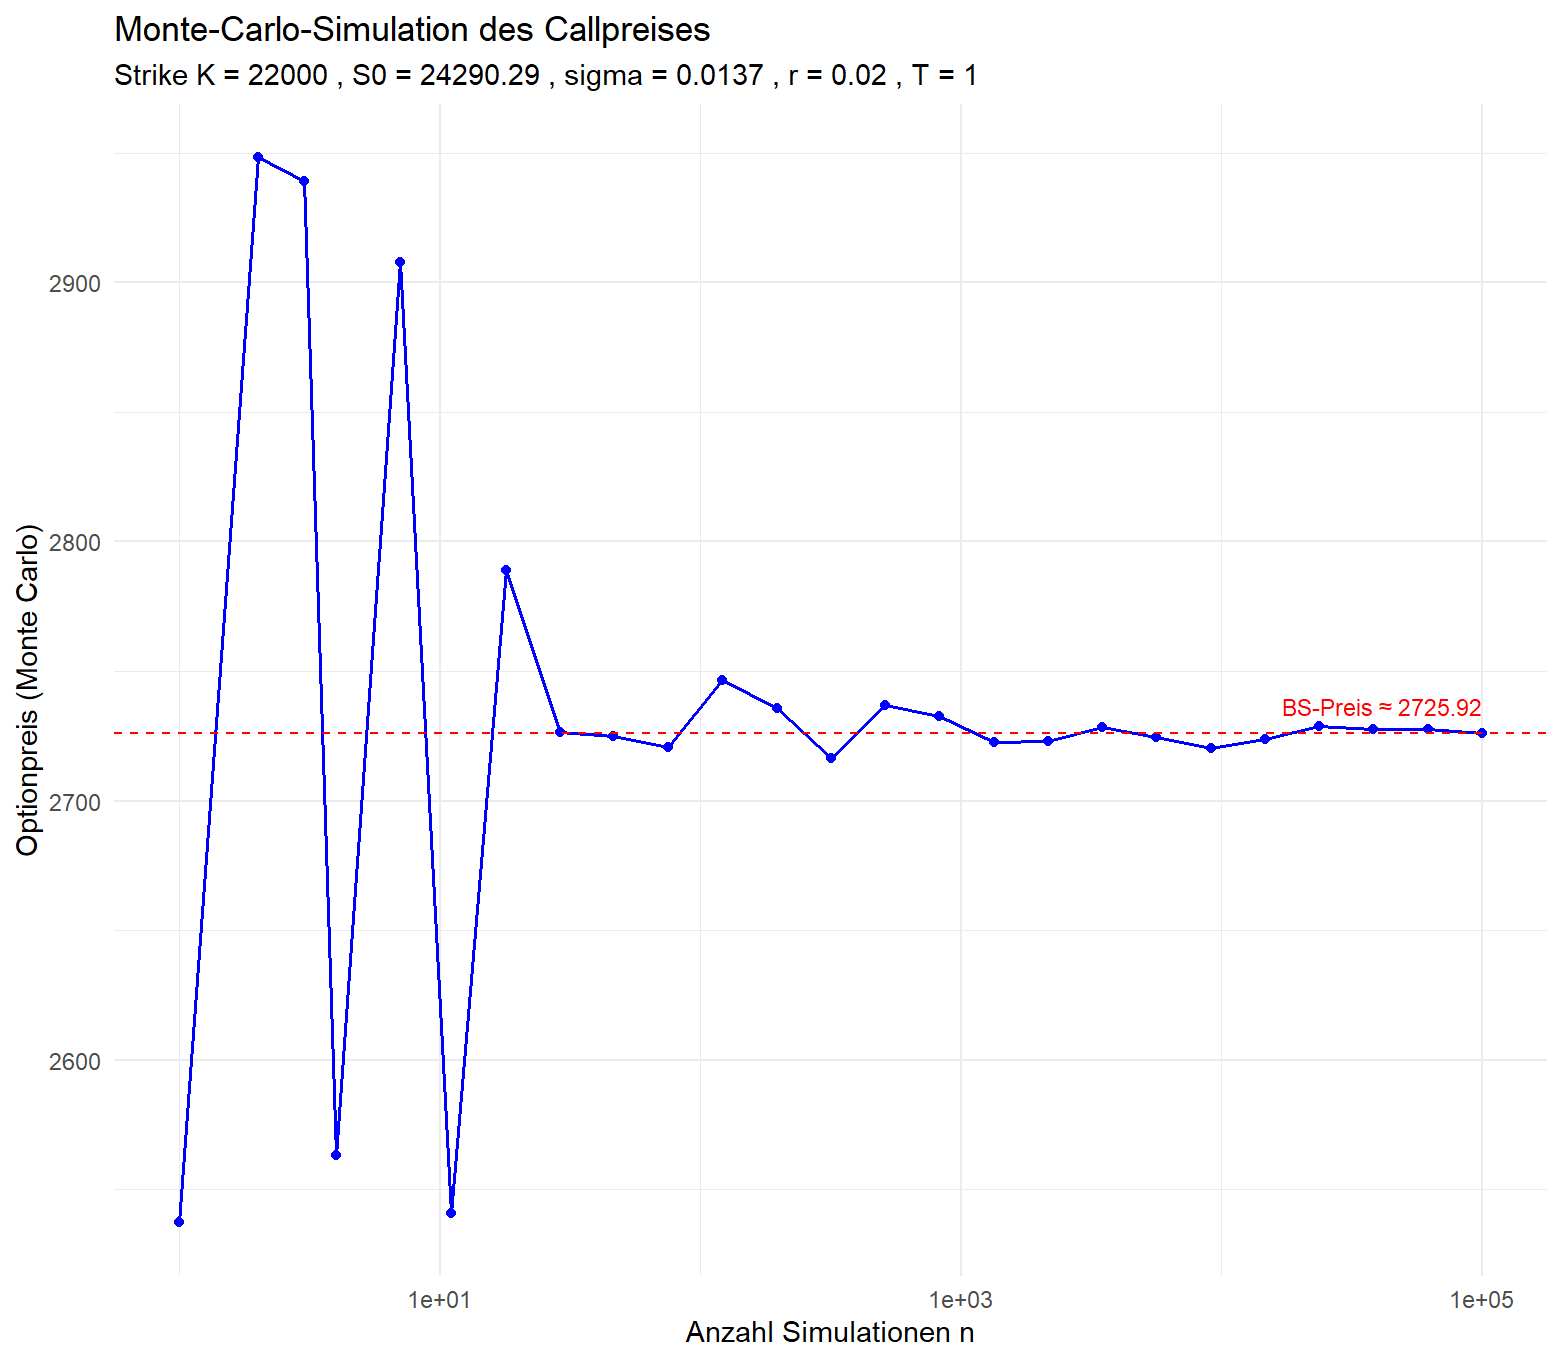
\includegraphics[width=0.48\textwidth]{../thesis/images/call_dax_mc.png}
  \end{figure}
\end{frame}

\section{Ende}

\begin{frame}{Ausblick}
  \begin{itemize}
    \item Stochastische Differentialgleichungen
  \end{itemize}
\end{frame}

\begin{frame}{Schlusswort}
  \centering
  \Huge Vielen Dank für Ihre Aufmerksamkeit\\
\end{frame}

\end{document}